\section{Fundamentals}

\begin{frame}
    \frametitle{Fundamentals - GAN}

    \begin{center}
        What are Generative Adversarial Networks?
        
        \begin{figure}[H]
            \centering
            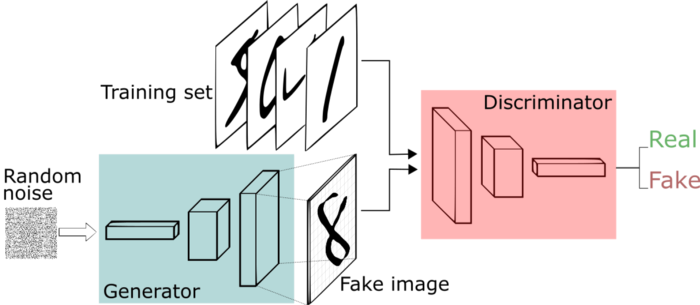
\includegraphics[width=0.65\textwidth]{resources/images/gan.png}
            \caption{Illustration of the general architecture of a Generative Adverserial Network. By \citeauthor{twd:gan} \cite{twd:gan}.}
            \label{fig:gan}
        \end{figure}
    \end{center}
\end{frame}

\begin{frame}
    \frametitle{Fundamentals - GAN}

    \begin{center}
        First GAN by \citeauthor{goodfellow2014generative} \cite{goodfellow2014generative}
    
        \begin{equation}
            \min _{G} \max _{D} V(D, G)=\mathbb{E}_{\boldsymbol{x} \sim p_{\text {data }}(\boldsymbol{x})}[\log D(\boldsymbol{x})]+\mathbb{E}_{\boldsymbol{z} \sim p_{\boldsymbol{z}}(\boldsymbol{z})}[\log (1-D(G(\boldsymbol{z})))]
        \end{equation}
    \end{center}
\end{frame}

\begin{frame}
    \frametitle{Fundamentals - DCGAN}

    \begin{center}
        DCGAN Architecture
        
        \begin{figure}[H]
            \centering
            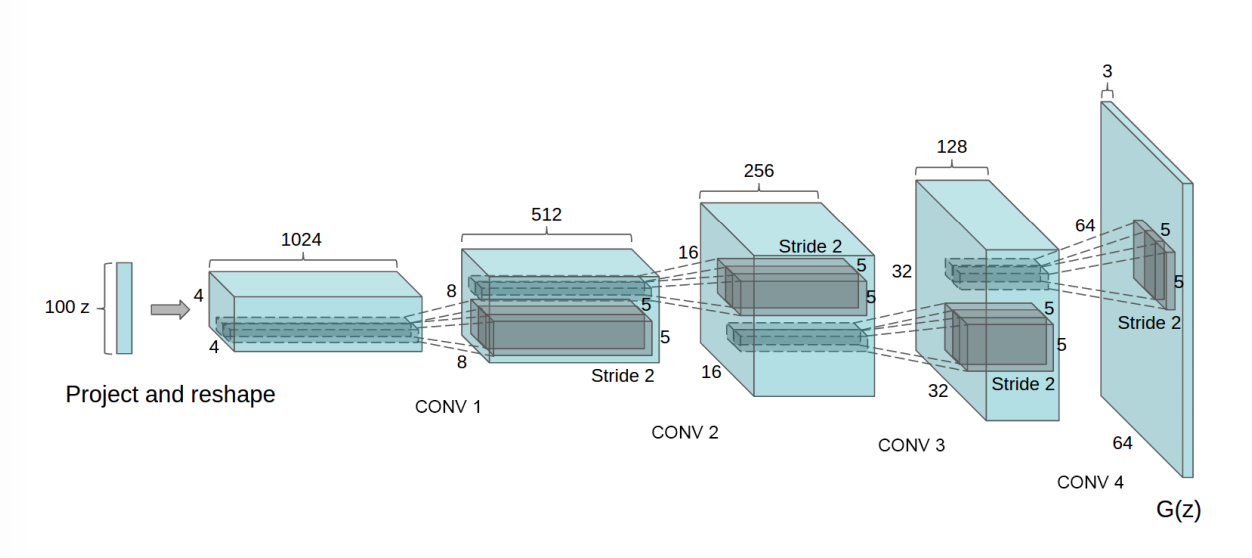
\includegraphics[width=0.65\textwidth]{resources/images/dcgan_generator.png}
            \caption{The Generator architecture proposed by \citeauthor{radford2016dcgan} in \citetitle{radford2016dcgan} \cite{radford2016dcgan}.}
            \label{fig:dcgan_generator}
        \end{figure}
    \end{center}
\end{frame}


\begin{frame}
    \frametitle{Fundamentals - WGAN}

    \begin{center}
        \begin{itemize}
            \item Other GANs losses approximate Kullback–Leibler or Jensen–Shannon divergence
            \item WGAN approximates the Earth-Mover's distance
            \item Requires a Lipschitz-1 continuous Discriminator
        \end{itemize}
    \end{center}
\end{frame}


\begin{frame}
    \frametitle{Fundamentals - WGAN}

    \begin{center}
        \begin{figure}[H]
            \centering
            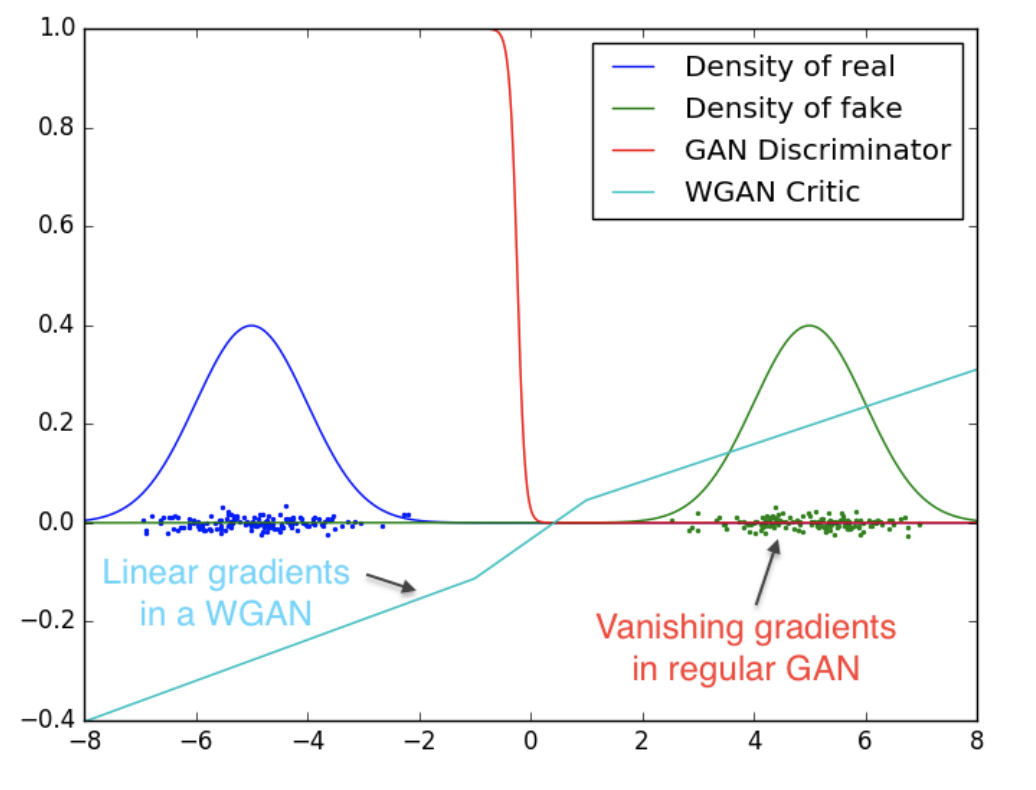
\includegraphics[width=0.65\textwidth]{resources/images/wgan1.png}
            \caption{The picture shows how WGAN performs compared to traditional GAN. WGAN can deliver strong gradients even if the two distributions do not overlap. The gradient signal vanishes for GANs.}
            \label{fig:wgan1}
        \end{figure}
    \end{center}
\end{frame}


\begin{frame}
    \frametitle{Fundamentals - Lipschitz Continuity}

    \begin{center}
        \begin{itemize}
            \item Requirement for WGAN loss
            \item Function is continuous at any point within a given interval
            \item Maximum absolute change between two consecutive steps must not be greater than $ L $
            \item Maximum absolute derivate at any point of the function is never higher than $ L $
            \item Solution: Weight-Clipping or Gradient Penalty
        \end{itemize}
    \end{center}
\end{frame}


\begin{frame}
    \frametitle{Fundamentals - Gradient Penalty}

    \begin{center}
        Additional regularization term for the Discriminator loss
        
        \begin{equation}
            \lambda \underset{\hat{x} \sim \mathbb{P}_{\hat{x}}}{\mathbb{E}}\left[\left(\left\|\nabla_{\hat{\boldsymbol{x}}} f(\hat{\boldsymbol{x}})\right\|_{2}-1\right)^{2}\right]
        \end{equation}\\
        
        Regularizes the Discriminator to have gradients with the norm of 1 almosteverywhere
    \end{center}
\end{frame}
